\begin{figure*}[t]
  \centering
  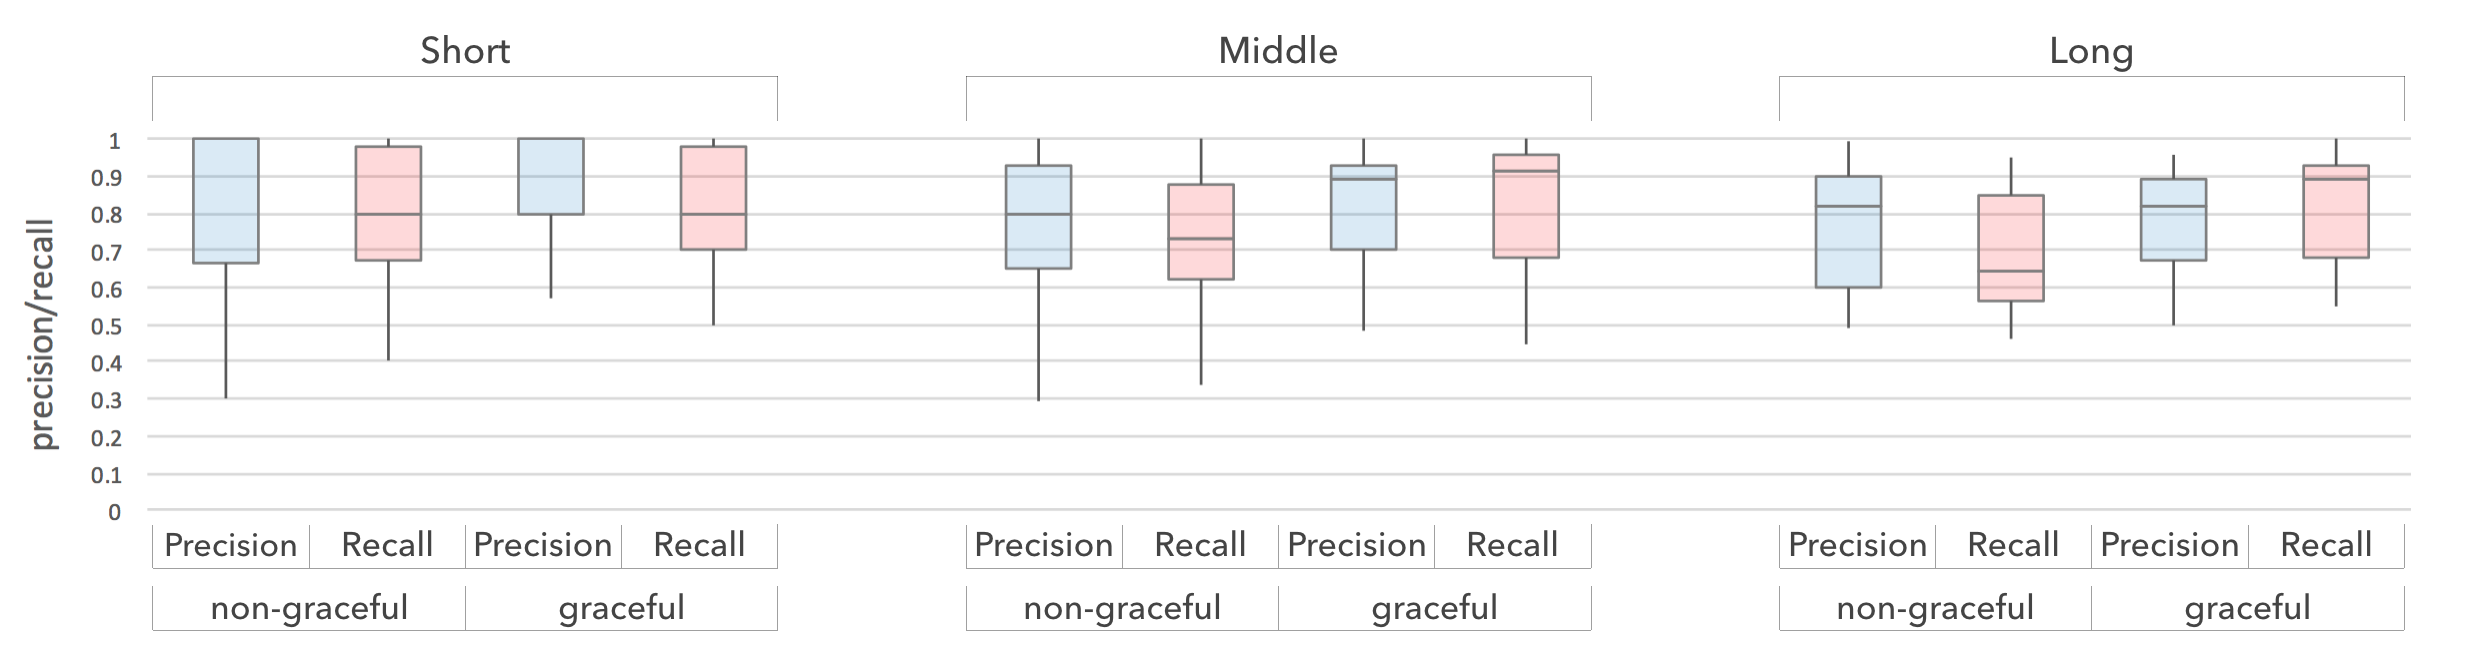
\includegraphics[width=2.0\columnwidth]{evaluate/difftrack_eval_commit.png}
  \caption{graceful matchingのコード断片の特定精度の評価の結果.\textit{Short}グループの適合率は,graceful matchingを用いた場合,用いなかった場合の両方において中央値が1.0であった.}~\label{fig:Commit_Matching_Accuracy_Evaluation}
%   \caption{Box plots of code matching accuracy performance results with our backtrack algorithm. Note that the medians for the precision under the \textit{Short} condition were 1.0 both with and without graceful matching.}~\label{fig:Commit_Matching_Accuracy_Evaluation}
  \vspace{-5mm}
\end{figure*}

\subsection{改良アルゴリズムの定量的評価}

graceful matchingが目的コード断片の特定の精度をどの程度改善するのかを明らかにするために,我々はGitHubの実際のコード変更データを用いた定量的評価を行った.
評価に用いるデータセットは,1,000人以上の開発者からスターを付けられており,かつデータセット構築時に最も新しく更新のあったChart.jsのリポジトリを選択した.
はじめにChart.jsのリポジトリから100個のコード断片を選択し,それらを\textit{Short}(9行以下,34個のコード変更),\textit{Middle}(10行以上30行以下,33個のコード変更),そして\textit{Long}(31行以上,33個のコード変更)の3つのグループに分類した.
次にそれら100個の原コード断片の開発履歴を辿り,5つ以上の過去のバージョンにおけるコード断片を抽出し,原コード断片と組み合わせる事で評価用のデータセットを構築した.
そして,過去のコード断片を特定する精度をgraceful matchingの有無で比較評価した.


% To understand how much the graceful matching improves target code piece identification, we conducted a quantitative evaluation using real code revision data obtained from open source repositories on GitHub.
% % We have two objectives for our evaluations: 1) to quantify how accurately the algorithm can estimate a code piece; and 2) to quantify how accurately the algorithm can extract a set of commits given a code piece.
% We chose 100 code pieces with various length of changes from the Chart.js repository, and divided into three groups: 34 \textit{Short} ($\sim 9$ lines), 33 \textit{Middle} ($10 \sim 30$ lines), and 33 \textit{Long} ($30 \sim$ lines).
% We then manually traced back the development history, and created the ground truth data consisting of more than five commits associated with each original source code piece.
% We evaluated the accuracy of selected commits with and without the graceful matching.

評価指標として適合率($P_{cp}$)と再現率($R_{cp}$)を用いた.
$l_c$を$\widehat{CP_{T}}$として正しく推定されたのコード行数,$l_i$を$\widehat{CP_{T}}$として間違って推定されたコードの行数,$l_n$を$CP_{T}$に含まれるが$\widehat{CP_{T}}$には含まれてないコードの行数とした時,適合率と再現率は$P_{cp} = \frac{l_c}{l_c + l_i},\;\; R_{cp} = \frac{l_c}{l_c + l_n}$と定義した.  

% We used precision and recall ($P_{cp}$, $R_{cp}$) as performance metrics.
% More specifically, $P_{cp} = \frac{l_c}{l_c + l_i},\;\; R_{cp} = \frac{l_c}{l_c + l_n},$ where $l_c$, $l_i$, and $l_n$ represent the numbers of lines correctly included in $\widehat{CP_{T}}$; lines incorrectly included in $\widehat{CP_{T}}$; and lines that are in $CP_{T}$ but not in $\widehat{CP_{T}}$, respectively.

図~\ref{fig:Commit_Matching_Accuracy_Evaluation}が示すように,全ての条件においてgraceful matchingを用いることで適合率と再現率が改善された.
また,適合率及び再現率の結果とgraceful matchingの有無に対して重回帰分析を行った結果,適合率と再現率が有意に改善されたことが分かった.
適合率における回帰係数は0.058($SE=0.025$, $p<.05$),再現率における回帰係数は0.051($SE=0.021$, $p<.05$)であった.
さらに,\textit{Short}グループの方が\textit{Long}のグループと比較して,有意に高い適合率及び再現率であった($p<.05$).

% Figure~\ref{fig:Commit_Matching_Accuracy_Evaluation} summarizes the results, showing that the performance was high across all the conditions.
% We ran multi-level linear regression analysis with two factors: the length group and the presence of graceful matching.
% The result showed that graceful matching significantly improved precision and recall.
% The estimated coefficients were 0.058 ($SE=0.025$, $p<.05$) and 0.051 ($SE=0.021$, $p<.05$) for precision and recall, respectively.
% \textit{Short} also showed significantly higher precision and recall than \textit{Long} ($p<.05$).

graceful matchingの評価を行った結果,コード断片の特定における適合率および再現率を約5\%改善できたことが分かった.
また図~\ref{fig:Commit_Matching_Accuracy_Evaluation}に示すように,graceful matchingが頑健性に貢献することが示された.
例えば,ある1つのデータでは,LHDiffのみの場合適合率と再現率がそれぞれ0.30と0.40であったが,graceful matchingを適用することで両方ともに0.80まで改善したことが確認された.
graceful matchingはコード断片の特定の精度を改善することができるため,我々はgraceful matchingをCodeGlassに導入することとした.

% The results suggest that our graceful approach can improve precision and recall of identifying commits by roughly 5\% in our dataset.
% Although the effect estimated by our multi-level linear regression was not large, it offers robustness to cases in which the default backtrack algorithm exhibits low precision and recall as shown in Figure~\ref{fig:Commit_Matching_Accuracy_Evaluation}.
% In one test case, the na\"{i}ve LHDiff algorithm was only able to achieve the precision and recall of 0.30 and 0.40, respectively, but the graceful approach improved both of them to 0.80.
% We thus concluded that the graceful approach can improve commit matching and should be included in the CodeGlass system.





